\section{Calculating the attributes}

Before we can properly print results in the program, we need to calculate the attributes of the different routes.
This is a relatively difficult task, as we need to calculate the distance, price, \unit{CO_{2}} and comfort.
Some attributes are easier to calculate than others, but they all require some form of calculation.

Rejseplanen has systems in place to calculate some of those attributes, but the API does not provide them.
This means that we have to calculate them ourselves.
Our calculations will not be 100\% accurate, but they will be close enough for our purposes.

\subsection{Calculating distance}

As we don't use a map API, we can't properly calculate the distance between two points.
This means that we have to ignore roads and instead calculate the distance by the train tracks.
The problem is that Rejseplanen only provides the coordinates of the stations, not the tracks.
So what we decided to do instead is to calculate the distance between the stations.
This won't account for curves along the track, as the distance is calculated as a straight line between the stations.
However, doing this for every station along the route is better than doing this for only the start and end station.
You can see an example of how the distance is going to look in Figure~\ref{fig:image-google-maps-distance-calculation}.

\begin{figure}[H]
    \centering
    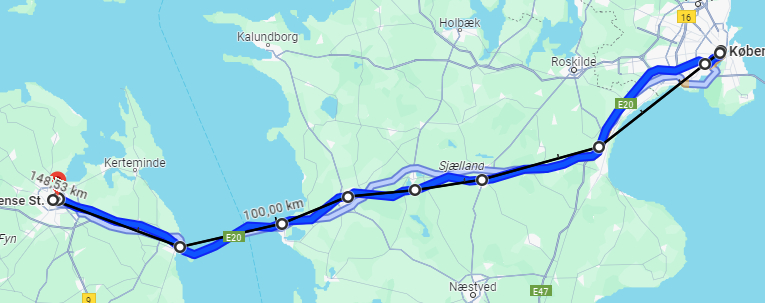
\includegraphics[width=0.8\textwidth]{images/google-maps-distance-calculation.jpg}
    \caption{A route between Copenhagen and Odense. \\ Blue line is Google Maps' distance, black line is our distance.}
    % TODO fix the text not being centered
    \label{fig:image-google-maps-distance-calculation}
\end{figure}

% TODO Add explanation for how we calculate the distance

\subsection{Calculating price}

Calculating the price is a lot more difficult than calculating the distance.
As Denmark is divided into zones, the price is calculated based on how many zones you travel through.
The price is also affected based on a number of different variables, such as age, region, occupation and more.
For our program, we decided to calculate the prices for Pendlerkort and Ungdomskort.

\subsubsection{Zones}

First thing we need to do is to figure out how many zones a route goes through.
Unfortunately, Rejseplanen's API does not provide any information about how many zones a route goes through.
What we decided to do instead is to find the average size for a zone.
As the zones are not all the same size, the number of zones a route passes through may be slightly off.
But this is the best we can do with the current circumstances.

First we started by picking two stations and counted how many zones the route goes through using DSB's zone
map~\cite{price_zones}.
We then used Google Maps to calculate the distance along the tracks between two stations, and we noted it down.
Finally, we divided the distance by the number of zones to get the average size of a zone along the route.

\begin{figure}[H]
    \centering
    \noindent
    \begin{tabular}{ || c | c | c || }
        \hline
        Route & Zones and distance & Zone size \\
        \hline\hline
        Korsør to Ringsted & 5 zones 45 km & 9 km per zone \\
        \hline
        Ringsted to Køge Nord & 6 zones 30 km & 5 km per zone \\
        \hline
        Kalundborg to Holbæk & 7 zones 45 km & 6.4 km per zone \\
        \hline
        Frederikssund to Kbh & 10 zones 23 km & 2.3 km per zone \\
        \hline
        Voldingborg to Ringsted & 8 zones 52 km & 6.5 km per zone \\
        \hline\hline
        Zone Averages & & 6 km per zone \\
        \hline
    \end{tabular}
    \caption{Table of our calculations of zone size averages.}
    \label{fig:table-zone-size-averages}
\end{figure}

From Figure~\ref{fig:table-zone-size-averages} we determined that the average size of a zone is roughly about 6
kilometers.
But as you can see, the sizes of zones varies a lot.
This is unfortunate for us, as it means that the number of zones a route goes through may be inaccurate.

\subsubsection{Pendlerkort price}

The way we're going to calculate the price will is by figuring out the price for Pendlerkort.
This card allows commuters to freely travel between set amount of zones.
Rejseplanen has a website where the user can input their route, and it'll calculate the price for the
Pendlerkort~\cite{price_calculator}.
We then took the results and compared them to the price chart provided by DSB~\cite{price_sheet}.
Our calculations can be found in Figure~\ref{fig:table-rejseplanen-price-calculations} and
Figure~\ref{fig:image-dsb-pendlerkort-pris}.
The results are accurate enough that we deemed them good enough for our purposes.

\begin{figure}[H]
    \centering
    \noindent
    \begin{tabular}{ || c | c || }
        \hline
        Route & Zones and price \\
        \hline\hline
        Odense to København & 30 zones 3750 kr \\
        \hline
        Køge Nord to København & 9 zones 1470 kr \\
        \hline
        Græsted to Vordingborg & 18 zones 3000 kr \\
        \hline
        Aarhus to København & 51 zones 4590 kr \\
        \hline
    \end{tabular}
    \caption{Table of Rejseplanen's price calculations.}
    \label{fig:table-rejseplanen-price-calculations}
\end{figure}

\begin{figure}[H]
    \centering
    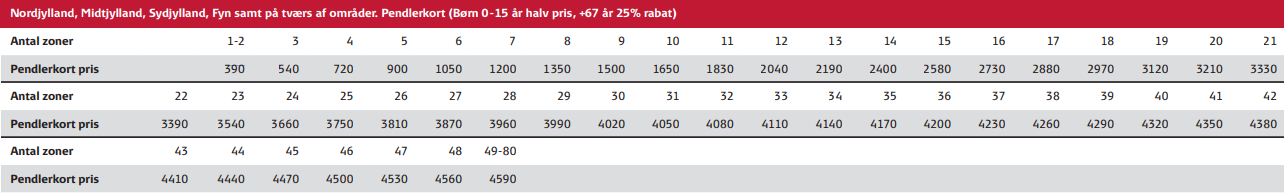
\includegraphics[width=1\textwidth]{images/dsb-pendlerkort-pris.jpg}
    \caption{Price of Pendlerkort per zones.}
    \label{fig:image-dsb-pendlerkort-pris}
\end{figure}

From what it seems, the price table is not recursive, so we can't implement a function to calculate the price.
Instead, we can save the table in the program and reference it when we need to find the price.
This allows us to have a pretty accurate price chart as long as the number of zones is accurate.

\subsubsection{Ungdomskort price}

Ungdomskort is a type op Pendlerkort that is primarily aimed at young people or students.
The price is significantly lower than Pendlerkort, so we deemed it necessary to implement it in our program.
The program would ask the user if they're a student, and if they are, the next calculation will be executed.
Calculating the price for Ungdomskort is a lot easier than Pendlerkort, as the method is listed on their
website~\cite{price_ung}.

The price is calculated by taking the equivalent price for a Pendlerkort and then taking 2487 kr from it.
Then the result is halved, and finally 663 kr is added to the result.
Here's an example for a Pendlerkort between Odense and Copenhagen, that costs 3750 kr:

\begin{equation}
    \frac{3750 - 2487}{2} + 663 = 1294 kr
\end{equation}

As a member in our group travels that same distance with an Ungdomskort, we can confirm that this result is accurate.

% textidote: ignore begin
\subsection{Calculating \unit{CO_{2}} emission}
% TODO Add the calculations, remove textiodte ignore
% textidote: ignore end

% textidote: ignore begin
\subsection{Calculating comfort value}
% TODO Add the calculation, remove textiodte ignore
% textidote: ignore end
